\documentclass[]{foi} 

\usepackage[utf8]{inputenc}
\usepackage{lipsum}
\usepackage{listings}
\usepackage{xcolor}
\usepackage{graphicx}
\usepackage{float}
\usepackage{longtable}
\usepackage{tikz}
\usetikzlibrary{shapes,arrows,positioning,fit,backgrounds}

% KOD STYLING
\lstset{
    language=Python,
    basicstyle=\ttfamily\footnotesize,
    commentstyle=\itshape\color{gray},
    keywordstyle=\color{blue}\bfseries,
    stringstyle=\color{red},
    showstringspaces=false,
    breaklines=true,
    prebreak=\raisebox{0ex}[0ex][0ex]{\ensuremath{\hookleftarrow}},
    numbers=left,
    numberstyle=\tiny\color{gray},
    stepnumber=1,
    backgroundcolor=\color{white},
    frame=single,
    rulecolor=\color{black},
    captionpos=b
}

\vrstaRada{\projekt}

\title{Top-Down Survival Shooter sa ZODB i PyGame}
\predmet{Baze Podataka}

\author{Student Studentić} 
\spolStudenta{\musko} 

\mentor{Dr. sci. Imetor Prezimento}
\spolMentora{\musko} 
\titulaProfesora{prof.~dr.~sc.}

\godina{2026}
\mjesec{siječanj}

\indeks{12345678}

\smjer{Informacijski i poslovni sustavi}


\sazetak{Ovaj projekt prikazuje razvoj računalne igre žanra Top-Down Survival Shooter korištenjem objektno-orijentirane baze podataka ZODB i PyGame frameworka za grafičko sučelje. Glavni cilj projekta je demonstrirati prednosti korištenja objektne baze podataka za perzistenciju velikog broja dinamičkih objekata (poput metaka i neprijatelja), izbjegavajući pritom problem nepodudarnosti impedancije (impedance mismatch) karakterističan za relacijske baze. Aplikacija implementira sustav za praćenje igrača, aktivnih projektila, neprijatelja i rezultata (High Scores). Poseban naglasak stavljen je na implementaciju ACID transakcija, korištenje B-stabala (BTree) za indeksiranje rezultata, te implementaciju poslovne logike kroz metode modela i "property" settere koji djeluju kao okidači (triggers). Rezultat je robusna aplikacija koja transparentno sprema stanje stotina objekata u \texttt{.fs} datoteku.}

\kljucneRijeci{ZODB; objektne baze podataka; PyGame; Survival Shooter; Python; perzistencija; transakcije; okidači; BTree}

\acrodef{ZODB}{Zope Object Database}
\acrodef{TDSS}{Top-Down Survival Shooter}
\acrodef{OOBP}{Objektno-orijentirana baza podataka}
\acrodef{ACID}{Atomicity, Consistency, Isolation, Durability}

% FIX za longtable i colortbl konflikt
\makeatletter
\providecommand\LT@@hline{}
\makeatother

\begin{document}

\maketitle

\tableofcontents

\makeatletter \def\@dotsep{4.5} \makeatother
\pagestyle{plain}

\chapter{Uvod}

\section{Opis Aplikacijske Domene}
Računalne igre su kompleksni softverski sustavi koji zahtijevaju upravljanje velikim brojem stanja u stvarnom vremenu. U žanru \ac{TDSS} igara, stanje uključuje veliki broj aktivnih entiteta koji se brzo mijenjaju: pozicije stotina metaka, koordinate neprijatelja koji nadiru u valovima, te stanje igrača (zdravlje, \textit{power-up} statusi). Tradicionalni pristup korištenjem relacijskih baza podataka zahtijeva mapiranje svakog metka ili neprijatelja u redak tablice, što je iznimno neefikasno za ovakav tip "živog" sustava.

Ovaj projekt implementira jednostavnu 2D \ac{TDSS} igru gdje igrač upravlja likom, bori se protiv hordi neprijatelja i skuplja \textit{power-up} predmete. Svi podaci o igri -- uključujući svaki ispaljeni metak i svakog neprijatelja na ekranu -- moraju biti trajno pohranjeni kako bi igrač mogao nastaviti igru točno tamo gdje je stao.

\section{Motivacija i Cilj}
Glavna motivacija za odabir \ac{ZODB} tehnologije je njezina sposobnost transparentne perzistencije Python objekata. Cilj je pokazati kako se objektna baza podataka može integrirati u petlju igre (Game Loop) te kako olakšava razvoj eliminirajući potrebu za SQL upitima i ORM (Object-Relational Mapping) slojevima.

\chapter{Teorijski okvir}

\section{Objektno-Orijentirane Baze Podataka (OOBP)}
Objektno-orijentirana baza podataka (\ac{OOBP}) pohranjuje podatke u obliku objekata, baš onako kako su predstavljeni u programskom jeziku. Ovo rješava problem \textit{impedance mismatch}-a, odnosno nesrazmjera između objektnog modela aplikacije i relacijskog modela baze podataka \cite{OOBP2015}. 

\ac{ZODB} je nativna objektna baza za Python koja pruža sljedeća svojstva:
\begin{itemize}
    \item \textbf{Transparentnost:} Objekti se automatski spremaju kada su promijenjeni.
    \item \textbf{ACID Transakcije:} Osiguravaju integritet podataka.
    \item \textbf{Povijest i Undo:} Mogućnost vraćanja na prethodna stanja.
\end{itemize}

\section{Usporedba s Relacijskim Pristupom}
Usporedba ZODB-a i klasičnih relacijskih baza (poput PostgreSQL-a) u kontekstu razvoja igara prikazana je u tablici \ref{tab:comparison}.

\begin{table}[h!]
    \centering
    \caption{Usporedba ZODB i Relacijskih baza}
    \label{tab:comparison}
    \begin{tabular}{|l|l|l|}
    \hline
    \textbf{Svojstvo} & \textbf{ZODB (Objektna)} & \textbf{PostgreSQL (Relacijska)} \\
    \hline
    Model podataka & Python klase i objekti & Tablice i redci \\
    \hline
    Upiti & Navigacija po grafu, BTree & SQL (SELECT, JOIN) \\
    \hline
    Odnosi & Direktne reference & Strani ključevi (Foreign Keys) \\
    \hline
    Perzistencija & \texttt{transaction.commit()} & SQL INSERT/UPDATE \\
    \hline
    Fleksibilnost & Visoka (promjena sheme) & Niska (ALTER TABLE) \\
    \hline
    \end{tabular}
\end{table}

\section{ACID Svojstva i Transakcije}
Sigurnost podataka u igri osigurana je ACID svojstvima \cite{ACID2020}:
\begin{itemize}
    \item \textbf{Atomarnost:} Cijela promjena stanja (npr. igrač pokupi predmet i dobije bodove) se sprema odjednom.
    \item \textbf{Konzistentnost:} Baza prelazi iz jednog validnog stanja u drugo.
    \item \textbf{Izolacija:} Ako bi igra podržavala više igrača, njihove transakcije se ne bi miješale.
    \item \textbf{Trajnost:} Jednom kada se napravi \texttt{commit}, podaci su sigurni na disku.
\end{itemize}

\chapter{Model Baze Podataka}

Za razliku od ER dijagrama kod relacijskih baza, model \ac{ZODB}-a najbolje se opisuje grafom objekata koji kreću od korijenskog (root) objekta. Slika \ref{fig:uml_diagram} prikazuje UML dijagram klasa implementiranih u sustavu.

\begin{figure}[H]
\centering
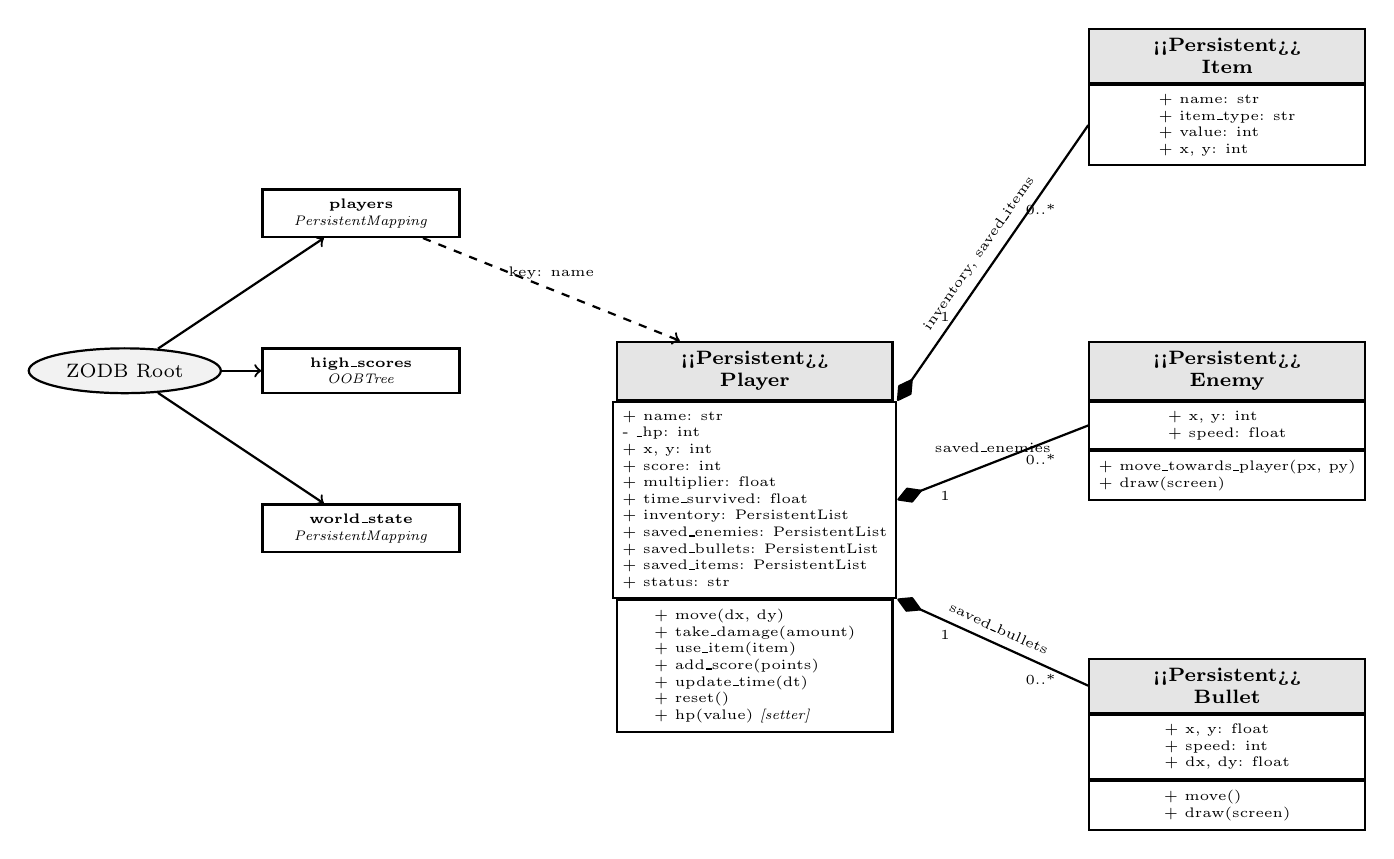
\begin{tikzpicture}[
  node distance=1.5cm,
  class/.style={
    rectangle, 
    draw=black, 
    fill=white,
    thick,
    minimum width=3.5cm, 
    align=center,
    font=\tiny
  },
  title/.style={
    font=\bfseries\scriptsize,
    align=center,
    minimum height=0.6cm,
    fill=gray!20,
    draw=black,
    thick,
    minimum width=3.5cm
  },
  note/.style={
    rectangle,
    draw=black,
    fill=yellow!10,
    dashed,
    font=\tiny,
    align=left,
    minimum width=2cm
  }
]

% --- ZODB ROOT STRUCTURE (Left Side) ---
\node[draw=black, ellipse, thick, fill=gray!10, font=\scriptsize] (root) at (-7, 0) {ZODB Root};

\node[class, minimum width=2.5cm] (mapping) at (-4, 2) {
    \textbf{players}\\
    \textit{PersistentMapping}
};

\node[class, minimum width=2.5cm] (btree) at (-4, 0) {
    \textbf{high\_scores}\\
    \textit{OOBTree}
};

\node[class, minimum width=2.5cm] (world) at (-4, -2) {
    \textbf{world\_state}\\
    \textit{PersistentMapping}
};

\draw[->, thick] (root) -- (mapping);
\draw[->, thick] (root) -- (btree);
\draw[->, thick] (root) -- (world);

% --- PLAYER CLASS (Center) ---
\node[title] (player_title) at (1,0) {<<Persistent>>\\Player};
\node[class, below=0pt of player_title, align=left] (player_attr) {
    + name: str\\
    - \_hp: int\\
    + x, y: int\\
    + score: int\\
    + multiplier: float\\
    + time\_survived: float\\
    + inventory: PersistentList\\
    + saved\_enemies: PersistentList\\
    + saved\_bullets: PersistentList\\
    + saved\_items: PersistentList\\
    + status: str
};
\node[class, below=0pt of player_attr, align=left] (player_methods) {
    + move(dx, dy)\\
    + take\_damage(amount)\\
    + use\_item(item)\\
    + add\_score(points)\\
    + update\_time(dt)\\
    + reset()\\
    + hp(value) \textit{[setter]}
};

% Connect Mapping to Player
\draw[->, thick, dashed] (mapping) -- (player_title) node[midway, above, font=\tiny] {key: name};

% --- RELATED CLASSES (Right Side) ---

% ITEM (Top Right)
\node[title] (item_title) at (7, 4) {<<Persistent>>\\Item};
\node[class, below=0pt of item_title, align=left] (item_attr) {
    + name: str\\
    + item\_type: str\\
    + value: int\\
    + x, y: int
};

% ENEMY (Middle Right)
\node[title] (enemy_title) at (7, 0) {<<Persistent>>\\Enemy};
\node[class, below=0pt of enemy_title, align=left] (enemy_attr) {
    + x, y: int\\
    + speed: float
};
\node[class, below=0pt of enemy_attr, align=left] (enemy_methods) {
    + move\_towards\_player(px, py)\\
    + draw(screen)
};

% BULLET (Bottom Right)
\node[title] (bullet_title) at (7, -4) {<<Persistent>>\\Bullet};
\node[class, below=0pt of bullet_title, align=left] (bullet_attr) {
    + x, y: float\\
    + speed: int\\
    + dx, dy: float
};
\node[class, below=0pt of bullet_attr, align=left] (bullet_methods) {
    + move()\\
    + draw(screen)
};

% --- RELATIONSHIPS ---
% Player <>-- Item (Inventory + Saved Items)
\draw[diamond-, thick] (player_attr.north east) -- (item_attr.west) 
    node[midway, above, sloped, font=\tiny] {inventory, saved\_items}
    node[near start, above, font=\tiny] {1}
    node[near end, below, font=\tiny] {0..*};

% Player <>-- Enemy (Saved Enemies)
\draw[diamond-, thick] (player_attr.east) -- (enemy_attr.west) 
    node[midway, above, font=\tiny] {saved\_enemies}
    node[near start, below, font=\tiny] {1}
    node[near end, below, font=\tiny] {0..*};

% Player <>-- Bullet (Saved Bullets)
\draw[diamond-, thick] (player_attr.south east) -- (bullet_title.west) 
    node[midway, above, sloped, font=\tiny] {saved\_bullets}
    node[near start, below, font=\tiny] {1}
    node[near end, below, font=\tiny] {0..*};

\end{tikzpicture}
\caption{UML Model podataka s prikazom ZODB hijerarhije}
\label{fig:uml_diagram}
\end{figure}

\section{Struktura Korijenskog Objekta}
Korijenski objekt (\texttt{db.root}) sadrži tri glavne kolekcije:
\begin{enumerate}
    \item \texttt{players} (\texttt{PersistentMapping}): Mapa koja čuva objekte igrača, gdje je ključ ime igrača.
    \item \texttt{high\_scores} (\texttt{OOBTree}): B-stablo za efikasno čuvanje i dohvaćanje najboljih rezultata. OOBTree je optimiziran za velike količine podataka i pretraživanje raspona.
    \item \texttt{world\_state} (\texttt{PersistentMapping}): Spremište za globalno stanje svijeta (npr. ime zadnjeg igrača).
\end{enumerate}

\section{Klase Podataka}

Glavni entiteti u sustavu su \texttt{Player} i \texttt{Item}. Obje klase nasljeđuju \texttt{Persistent} kako bi ih ZODB mogao pratiti.

\subsection{Klasa Player}
Predstavlja igrača u igri. Sadrži logiku kretanja, zdravlja i inventara.

\begin{longtable}{|l|l|l|}
\caption{Atributi klase Player} \label{tab:player_attr} \\
\hline
\textbf{Atribut} & \textbf{Tip} & \textbf{Opis} \\
\hline
\endfirsthead
\hline
\textbf{Atribut} & \textbf{Tip} & \textbf{Opis} \\
\hline
\endhead
\hline
\endfoot
\texttt{name} & string & Jedinstveno ime igrača (ID). \\
\hline
\texttt{\_hp} & int & Trenutno zdravlje (0-100). \\
\hline
\texttt{x, y} & int & Koordinate na ekranu. \\
\hline
\texttt{score} & int & Trenutni rezultat. \\
\hline
\texttt{multiplier} & float & Množitelj bodova (povećava se prikupljanjem). \\
\hline
\texttt{time\_survived} & float & Vrijeme preživljavanja u sekundama. \\
\hline
\texttt{inventory} & PersistentList & Lista prikupljenih predmeta. \\
\hline
\texttt{saved\_enemies} & PersistentList & Lista aktivnih neprijatelja (za save/load). \\
\hline
\texttt{saved\_bullets} & PersistentList & Lista aktivnih metaka (za save/load). \\
\hline
\texttt{saved\_items} & PersistentList & Lista ne-prikupljenih predmeta na mapi. \\
\hline
\texttt{status} & string & Stanje ("Active", "Defeated"). \\
\hline
\end{longtable}

\subsection{Klasa Item}
Predstavlja predmete koje igrač može pokupiti.

\begin{itemize}
    \item \texttt{name}: Naziv predmeta (npr. "Drop\_heal").
    \item \texttt{item\_type}: Tip predmeta ("heal" ili "score").
    \item \texttt{value}: Numerička vrijednost (količina liječenja ili bodova).
    \item \texttt{x, y}: Pozicija na mapi prije nego je pokupljen.
\end{itemize}

\chapter{Implementacija}

Aplikacija je implementirana u programskom jeziku Python koristeći \texttt{PyGame} biblioteku za grafiku i ulazne uređaje, te \texttt{ZODB} za sloj podataka.

\section{Arhitektura Sustava}
Projekt je podijeljen u module radi bolje organizacije:
\begin{itemize}
    \item \texttt{src/database.py}: Upravlja konekcijom prema \texttt{game.fs} datoteci i inicijalizira strukture.
    \item \texttt{src/models.py}: Definira klase podataka i poslovnu logiku.
    \item \texttt{src/main.py}: Sadrži \textit{Game Loop}, upravljanje događajima i iscrtavanje.
\end{itemize}

\section{Upravljanje Bazom (GameDB klasa)}
Klasa \texttt{GameDB} enkapsulira sve operacije nad bazom. Prilikom inicijalizacije provjerava postojanje \texttt{data/} direktorija i kreira potrebne strukture unutar \texttt{db.root} ako ne postoje.

\begin{lstlisting}[caption={Metoda za dohvat Top Score-ova koristeći BTree},label={lst:btree_query}]
def get_top_scores(self, limit=5):
    """ Vraca top rezultate koristeci BTree efikasnost"""
    items = list(self.root['high_scores'].items())
    
    # Sortiranje po bodovima (prvi element u tuple-u vrijednosti)
    items.sort(key=lambda x: x[1][0], reverse=True)
    
    # Formatiranje povrata: (name, score, time)
    return [(name, val[0], val[1]) for name, val in items[:limit]]
\end{lstlisting}

\section{Implementacija Okidača (Triggers)}
ZODB nema klasične SQL okidače, ali se oni elegantno implementiraju koristeći Python \textit{property} mehanizam. U klasi \texttt{Player}, postavljanje HP-a automatski provjerava uvjet poraza.

\begin{lstlisting}[caption={Implementacija okidača za promjenu statusa},label={lst:hp_trigger}]
@hp.setter
def hp(self, value):
    self._hp = min(100, max(0, value))
    # OKIDAC: Ako je HP 0, promijeni status u "Defeated"
    if self._hp == 0:
        self.status = "Defeated"  # Automatska promjena
    # Javljamo ZODB-u da spremi promjenu
    self._p_changed = True  
\end{lstlisting}

Ovaj pristup osigurava da je poslovna logika ("igrač je poražen ako je HP=0") centralizirana i ne može se zaobići, bez obzira na to koji dio koda mijenja HP.

\section{Game Loop i Transakcije}
Igra se odvija u beskonačnoj petlji koja obrađuje ulaze, ažurira stanje i iscrtava sliku. Spremanje u bazu (commit) se ne radi u svakom frame-u zbog performansi, već u ključnim trenucima:
\begin{enumerate}
    \item Prilikom izlaza iz igre.
    \item Prilikom ažuriranja High Score tablice (kraj igre).
    \item Na zahtjev korisnika (tipka ESC za povratak u meni).
\end{enumerate}

\chapter{Primjeri Korištenja}

\section{Instalacija i Pokretanje}
Aplikacija dolazi s instalacijskom skriptom \texttt{setup.py} koja instalira potrebne biblioteke definire u \texttt{requirements.txt}. Pokretanje igre vrši se naredbom:
\texttt{python src/main.py}

\section{Scenarij Igranja}
\begin{enumerate}
    \item \textbf{Početak:} Igrač pokreće igru. Ako je prvi put, kreira se novi lik "Igrac1" na poziciji (400, 300).
    \item \textbf{Akcija:} Igrač se kreće tipkama W, A, S, D i puca lijevim klikom miša.
    \item \textbf{Prikupljanje:} Ubijanjem neprijatelja (crveni krugovi) ispadaju predmeti (žuti kvadrati). Igrač ih skuplja prelaskom preko njih, čime se oni dodaju u \texttt{PersistentList} inventar i odmah primjenjuju (povećanje HP-a ili bodova).
    \item \textbf{Spremanje:} Igrač mora prekinuti igru. Pritiskom na 'ESC', igra se pauzira, vraća u meni i poziva se \texttt{transaction.commit()}.
    \item \textbf{Nastavak:} Sljedeći dan igrač ponovno pokreće igru. Lik se nalazi na točno istoj poziciji, s istim brojem bodova i istim inventarom kao prije gašenja.
    \item \textbf{Game Over:} Ako HP padne na 0, igra završava. Rezultat se upisuje u \texttt{high\_scores} B-stablo u bazi. Prikazuje se lista najboljih rezultata dohvaćena iz baze.
\end{enumerate}

\section{Resetiranje Baze}
Za potrebe testiranja ili novog početka, priložena je skripta \texttt{reset\_db.py} koja briše \texttt{.fs} datoteku i omogućuje čisti start.

\chapter{Zaključak}

\ac{ZODB} se pokazao iznimno efikasnim za razvoj kompleksne logike igre. Ključne prednosti koje su uočene tijekom razvoja su:
\begin{itemize}
    \item \textbf{Brzina razvoja:} Nema potrebe za pisanjem SQL shema i migracija. Dodavanje novog atributa u klasu \texttt{Player} automatski je podržano.
    \item \textbf{Prirodna reprezentacija:} Graf objekata u memoriji se preslikava 1:1 na disk.
    \item \textbf{Pouzdanost:} ACID transakcije osiguravaju da se inventar ne izgubi čak ni u slučaju rušenja aplikacije (pod uvjetom da je napravljen commit).
\end{itemize}

Ovaj projekt uspješno demonstrira da su objektne baze podataka validna i često superiorna alternativa relacijskim bazama za domene koje su inherentno objektne, kao što su računalne igre i simulacije.

\makebackmatter

\end{document}